\documentclass[pageno]{jpaper}
%replace XXX with the submission number you are given from the ASPLOS submission site.
\newcommand{\asplossubmissionnumber}{XXX}

\usepackage[normalem]{ulem}
\begin{document}

\title{6.867 Machine Learning Homework 1}

\date{}
\maketitle

\thispagestyle{empty}


\section{Gradient Descent}

In this section we implemented the gradient descent function with parameters of objective function, gradient function, initial guess, step size and the convergence criterion.

We tested our gradient descent function on a convex function, a negative gaussian, as well as a multivariate very non-convex function with multiple minima, the Rosenbrock function. The negative gaussian is shown in Figure 1 and the python implementation of the Rosenbrock function is shown in Figure 2.
For functions with one global minimum and no local minimum, the negative gaussian we tested, the initial guess does not have any affect on solution. It does however have an affect on the number of iterations to convergence. For function with multiple local minimum the initial guess has a large effect.  Due to the fact that this implementation of gradient descent only proceeds to traverse the graph down the negative of the gradient it will always converge at a local minimum unless the initial guess is on the path to the global minimum. This dependency on the initial guess could be solved by repeating this procedure of gradient descent multiple times with random restarts and taking the minimum values calculated. 


\begin{figure}[ht!]
\centering
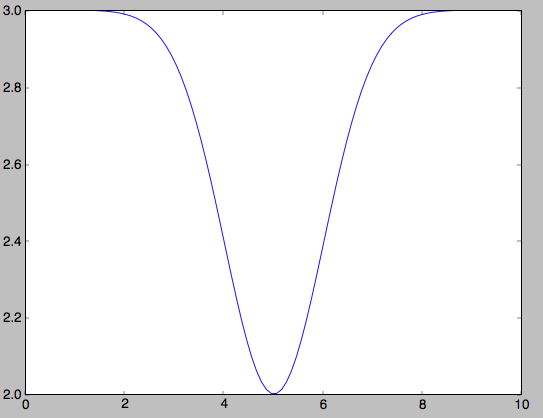
\includegraphics[width=60mm]{negative_gaussian}
\caption{Negative Gaussian}
\label{overflow}
\end{figure}

\begin{figure}[ht!]
\centering

\includegraphics[width=90mm]{rosenbrock}
\caption{Python implementation of Rosenbrock function}
\label{overflow}
\end{figure}

In table one below we investigate the effects of the step size and the convergence criterion on the final solution and number of iterations to convergence.
\begin{table}[h!]
  \centering
  \begin{tabular}{llllll|}
    \hline
    \textbf{Step Size}  & \textbf{Convergence Criterion}  & \textbf{No. Iterations} & \textbf{Error}\\
    \hline
    \hline
 0.0005 	&0.000001 &65114  &1.49 \\
 \hline
0.0005	&0.00001 	&46372 &0.791 \\
 \hline
0.0005	&0.0001 	&28371 &0.961 \\
 \hline
0.00005	&0.00001 	&285332 &0.363 \\
 \hline
0.005	&0.00001 	&Does Not Converge \\
 \hline
  \end{tabular}
  \caption{Step Size and Convergence Criterion vs. Number of Iterations to Convergence}
  \label{table:formatting}
\end{table}

In the table above we calculate the error as the actual minimum on the function minus the minimum calculated by gradient descent. 
As illustrated in our table, a smaller step size increases the number of iterations to convergence, due to the fact that we are moving at a smaller pace along the negative gradient toward the minimum. Too large of a step size will cause the gradient descent procedure to not converge. Additionally, a smaller step size does increase the accuracy of our results since we prevent moving along the gradient past the actual minimum. Similarly, a smaller convergence criterion increases the number of iterations needed for convergence. If we were to implement a line search technique as seen in Murphy eq. 8.11 we would be able to optimize our step size and improve performance.

We implemented an approximate to the the gradient function numerically at a given point using central differences. By comparing the analytical gradients that we used in the steps before and the numerical central differences gradient, we find that the numerical gradient is a much rougher estimate of the gradient. This is due to the fact that the analytical gradient is more exact as it is the derivative of the function while the numerical gradient is only an approximation to this gradient.

In table 2 we compare our simplistic gradient descent procedure with the numpy python implementation of the 
Broyden Fletcher Goldfarb Shanno optimization algorithm(scipy.optimize.fmin\_bfgs). We set the step size equal to 0.00005 and the convergence criterion to 0.00001.

\begin{table}[h!]
  \centering
  \begin{tabular}{llllll|}
    \hline
     \textbf{} & \textbf{Gradient Descent}  & \textbf{BFGS}  \\
     

    \hline
 Total Iterations &284942 	&3   \\
 \hline
 Function Evaluations &284842 	&75   \\
 \hline
 Gradient Evaluations &284842 &25\\
  \hline
Error &0.363 &.011\\
   \hline
  \end{tabular}
  \caption{Gradient Descent(step size = 0.00005, convergence =  0.00001) vs. BFGS}
  \label{table:formatting}
\end{table}
 
 As seen from the table 2 the BFGS algorithm is much quicker to convergence, computes fewer gradients and is more exact than our implementation of gradient descent. We tested our implementation on a negative gaussian and with the same initial starting point. 
 
\section{Linear Basis Function Regression}

In this section we explored linear basis regression functions and tested them on graphs provided in Bishop 1.4.

We computed the maximum likelihood weight vectors give an array of 1-d points, a vector of Y values and the value M(the maximum order of a simple polynomial basis function. To compute the maximum likelihood weight vectors we first computed the design matrix containing x(1.....n) as the columns and x to the power M as the rows.Finally we computed the regression fit weight vectors using the psuedoinverse of the design matrix. We replicated the plots in Bishop 1.4 as shown in figure 3. Table 3 shows the weight vector resulting from our implementation as well as the weight vector from Bishop 1.1 (comparison done for M=9). Our results are very close to agreement with those from Bishop.
\begin{figure}[ht!]
\centering
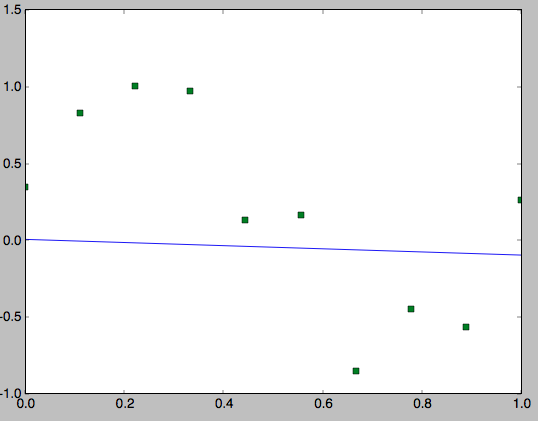
\includegraphics[width=60mm]{M_1}
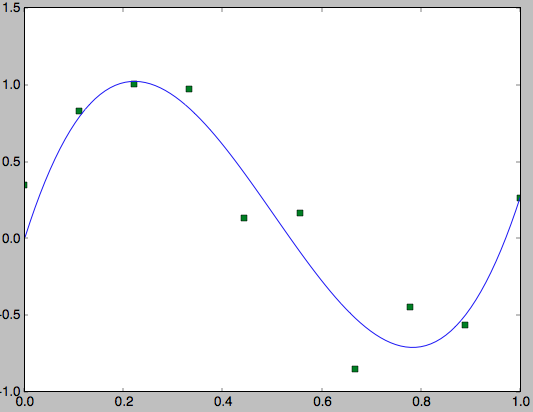
\includegraphics[width=60mm]{M_4}
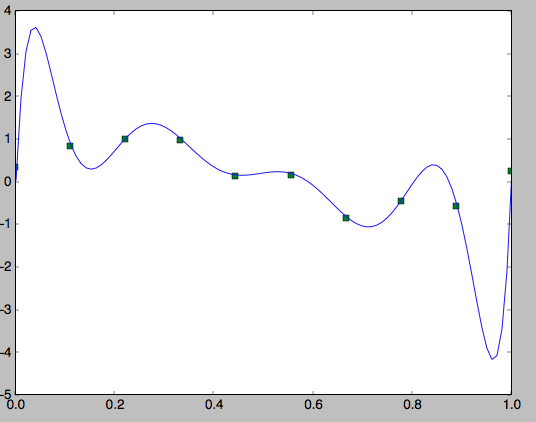
\includegraphics[width=60mm]{M_2}
\caption{Reproduction Of Bishop 1.4 plots (M =0, 1, 9)}
\label{overflow}
\end{figure}

\begin{table}[h!]
  \centering
  \begin{tabular}{llllll|l}
    \hline
    \textbf{w} & \textbf{Our Results}  & \textbf{Bishop Results}  \\
    \hline
    \hline
 0 	&0.00 &0.35 \\
 \hline
1	&241.26 	&232.37 \\
 \hline
2	&-5413.27 	&-5321.83  \\
 \hline
3	&4907.61 	&48568.31 \\
 \hline
4	&-233339.75 	&-231639.30 \\
 \hline
5	&643636.97 	&640042.261 \\
 \hline
6	&1066631.56 	&-1061800.52 \\
 \hline
7	&1046402.33 	&1042400.18 \\
 \hline
8	&-559545.74 	&-557682.99  \\
 \hline
9	&125573.92 	&125201.43 \\
 \hline
  \end{tabular}
  \caption{Computed Weight vector vs. Bishop Weight vector for M = 9}
  \label{table:formatting}
\end{table}

We calculated the gradient descent on the sum of squared errors function. Similar to what we saw in Section 1, the initial guess, convergence and step size had a sizable impact on the optimization problem. Small step sizes increased the number of iterations required for convergence but also increased the accuracy of the result. Too small of a step size would lead to the optimization problem never converging. Large step sizes tended to converge much quicker but lost on accuracy. Additionally, in theory, larger step sizes could move past a local or global minimum. A small convergence criterion lead to an increase in the number of iterations. This is simply due to the fact that a smaller convergence criterion means that the gradient descent must be run more iterations to reduce the error below this threshold. 
Additionally, we also compared our gradient descent on sum of squares function to the BFGS optimization function implementation in python(scipy.optimize.fmin\_bfgs). If the function being optimized is convex then both the sum of squares method and the BFGS method will have low error, due to the fact that there will be only one minimum, the global one. If the function is non-convex then the BFGS greatly outperforms the sum of squares optimization. Gradient descent can easily converge to a local optima while BFGS has more complex methods to dissuade against this. Similarly, the initial value plays a large role in the error of the gradient descent function and a much smaller role in that of the BFGS function. In the case of gradient descent, if the initial value is not chosen properly the function will converge to a local rather than global minima. 
In figure 4, we replicate the plot from Bishop 1.4 where M is equal to three. Notice that this implementation is less accurate than our original weight vector estimates using maximum likelihood.
\begin{figure}[ht!]
\centering
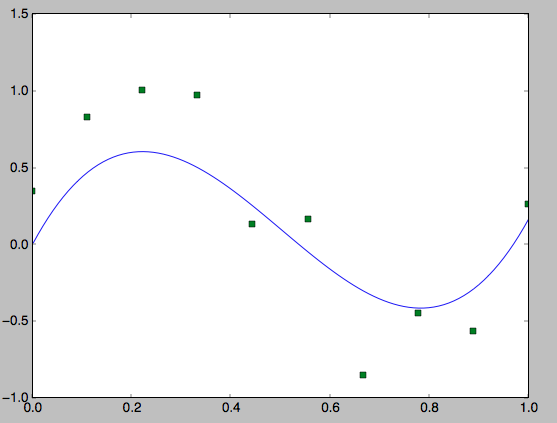
\includegraphics[width=60mm]{M_3}
\caption{Reproduction Of Bishop 1.4 plots (M =3) Using Sum of Squares}
\label{overflow}
\end{figure}

\section{Ridge Regression}
In this section we explore ridge regression. 
We explored the fit of the ridge regression function as we varied the values of M and lambda. Figure 5 contains three plots showing a comparison of two lambda values and of two M values. This is just a subset of the data we observed but conveys the necessary conclusions. As M decreases the error decreases. As lambda decrease the error decreases. Intuitively this makes sense because as lambda goes to zero the equation returns to the original linear basis function regression problem from section 2. 
\begin{figure}[ht!]
\centering
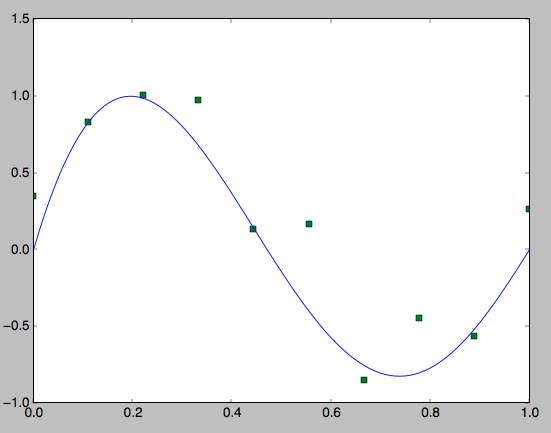
\includegraphics[width=60mm]{lambda=0001}
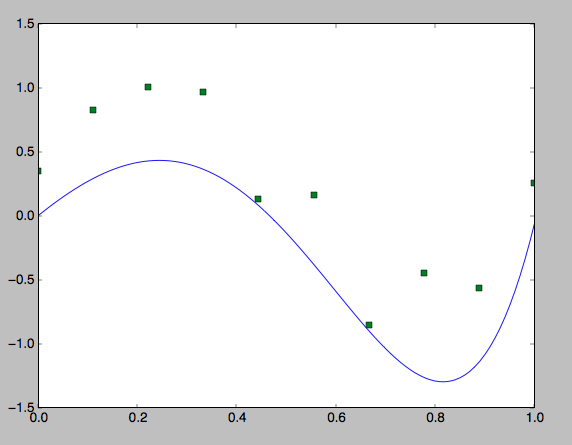
\includegraphics[width=60mm]{lambda=001}
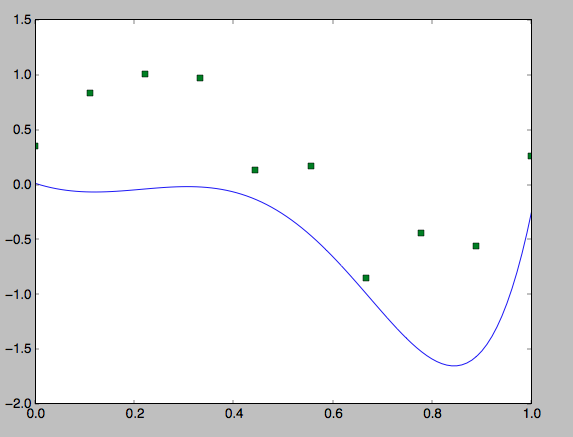
\includegraphics[width=60mm]{m=15}
\caption{Ridge Regression on Bishop 1.4, Top to Bottom, lambda = .0001, M = 5, lambda = .001, M =5, lambda = .001 and M = 14}
\label{overflow}
\end{figure}


We calculate the sum of squares error and we use this value as our error to optimize. We add in lambda into this error term so that when we minimize the sum of squares error for lambda we do not always get a value of zero. 

\begin{table}[h!]
  \centering
  \begin{tabular}{llllll|l}
    \hline
    \textbf{M} & \textbf{$\lambda$\ }  & \textbf{Training Set A}  & \textbf{Training Set B} & \textbf{Validation Set} \\
    \hline
 10 	&0.001 &2.916 &4.38 & 4.95\\
     \hline
 8 	&0.001 &4.26 &4.00 & 5.15\\
    \hline
 5 	&0.001 &3.13 &2.00 & 2.32\\
 \hline
  3 	&0.001 &0.826 &953.41 & 2.82\\
   \hline
  3 	&0.0001 &0.825 &546.86 & 2.75\\
 \hline
  3 	&0.00001 &0.825 &520.95 & 2.74\\
    \hline
  2 	&0.001 &6.5 &0.34 & 4.44\\
 \hline
 1 	&0.001 &1.43 &0.096 & 1.43\\
  \hline
 1 	&0.0001 &1.43 &0.088 & 1.43\\
\hline
 1 	&0.00001 &1.43 &0.087 & 1.43\\
\hline
 
  \end{tabular}
  \caption{Sum of Squares Errors on Training Set A, B and the Validation Set for various values of M and $\lambda$\   }
  \label{table:formatting}
\end{table}

Table 4 shows the sum of squares errors for a variety of M and $\lambda$\ values on training set A and B and the validation set. We can see from the experimentation that for training set A a value of M=3 and lambda = .00001 worked the best and for training set B a value of M = 1 and lambda = .00001 worked the best. For the validation set a value of M = 1 and lambda = .00001 worked the best. As lambda decreased we found that the errors decreased but at a diminishing rate(i.e. a drop in lambda by 10x only improved the error by .001).  The method we used to evaluate the best parameters is succeptible to falling into local minima and not reaching the global minima. We started out with high values of M and then tried lower values until we reached a minima and the next value was greater. This does not ensure the globally best values for the parameters, so there still may be more optimal solutions for the values of M and lambda.

\section{Generalizations}
In this section we investigate the effects of generalizations. Specifically we investigate the LAD and LASSO functions.
\begin{table}[h!]
  \centering
  \begin{tabular}{llllll|l}
    \hline
    \textbf{M} & \textbf{$\lambda$\ }  & \textbf{Training Set A}  & \textbf{Training Set B} & \textbf{Validation Set} \\
    \hline
 10 	&0.001 &1.71 &2.095 &2.23\\
     \hline
 8 	&0.001 & 2.045 &2.54 & 2.32\\
    \hline
 5 	&0.001 &1.77 & 1.41 & 1.52\\
 \hline
  3 	&0.001 &0.9 & 30.88 & 1.68\\
   \hline
  3 	&0.0001 &0.908 &23.39 & 1.66\\
 \hline
  3 	&0.00001 &0.90 & 22.82 & 1.65\\
    \hline
  2 	&0.00001 &2.55 & 0.58 & 1.65\\
 \hline
 1 	&0.001 &1.19 &0.31 & 1.19\\
  \hline
 1 	&0.0001 &1.19 &0.29 & 1.19\\
\hline
 1 	&0.00001 &1.19 &0.29 & 1.19\\
\hline
 \end{tabular}
  \caption{LAD on Training Set A, B and the Validation Set for various values of M and $\lambda$\   }
  \label{table:formatting}
\end{table}

The data in table 5 shows the results of running the gradient descent to find the weights of to minimize LAD and then evaluating with some values of M and lambda as we did in the previous section. Here we look to minimize the absolute values of the errors, the L1 norm, as opposed to the L2 norm in the previous examples. Compared to the ridge regression, the Training set A and B as well as the validation set are minimized by the same values of M and lambda.
\end{document}
